% use the base acmart.cls
% use the sigplan proceeding template with the default 10 pt fonts
% nonacm option removes ACM related text in the submission. 
\documentclass[sigplan,nonacm]{acmart}
\usepackage{csvsimple}

\newcommand{\fixme}[1]{\textcolor{red}{#1}}
\newcommand{\todo}[1]{\textcolor{red}{TODO:\ #1}}
\newcommand{\fullname}{More Exact Technology-Mapping using E-Graphs}
\newcommand{\shortname}{E-Pack}
\newcommand{\B}{\mathbb{Z}_{2}}
\newcommand{\Bk}{\mathbb{Z}_{2}^{k}}
\newcommand{\Bx}[1]{\mathbb{Z}_{2}^{#1}}

% enable page numbers
\settopmatter{printfolios=true}


\begin{document}

\title{\fullname}

\begin{abstract}
    FPGA technology mapping is a well-studied problem and has been an area of
    interest in EDA tool design for decades. In most respects, the computational
    complexity of technology mapping is understood, and heuristic algorithms have
    been successfully employed to mitigate compile times while maintaining high QoR
    (quality of results). As transistor scaling comes to an end within the coming
    years, logic synthesis tools will become more of a bottleneck in the design of
    high performance accelerators. As a solution, we introduce E-Pack, an e-graph
    driven technology mapper that can better span the wide gap between SAT-based
    exact synthesis and heuristic cut enumeration techniques. We show that E-Pack
    can synthesize circuits with 5\% fewer LUTs on average---without ever
    increasing circuit depth. We also provide an empirical analysis of the runtime
    of E-Pack and show that it is still practical for large designs. Finally, we
    demonstrate that our compiler infrastructure is reusable, and future work can
    use our compiler for RTL equivalence checking or auditing the QoR of synthesis
    tools.
\end{abstract}
\maketitle % should come after the abstract

\section{Introduction}\label{sec:intro}
Given the complexity of modern electronic systems, a high degree of automation
is required to develop custom hardware within sensible timelines. At the
highest level, FPGA and ASIC design flows can be split into logical synthesis
and physical synthesis (optimize timing, placement and routing, etc..). This
division of work produces suboptimal designs, and neither are the individual
synthesis steps locally optimal on their own. However, logic minimization
problems in general are NP-Hard~\cite{logicmin,twolevellogic}, and modern EDA
flows bring compile times down to the human timescale while maintaining
acceptable QoR (quality of results).

With the end of Moore's Law scaling, chip area becomes a tighter constraint,
and logic synthesis is more of a bottleneck. Hence, future synthesis tools will
need to expand the design spaces they explore and find more optimal solutions.
Nonetheless, finding provably optimal circuits is computationally intractable.
In this paper, we will introduce how FPGA technology mapping can be augmented
with e-graph data structures to find \textit{more} exact solutions, without
significantly increasing compile times.

Technology mapping is the hand-off between logical synthesis and physical
synthesis. It converts the abstract Boolean logic into a network of gates that
belong to the target cell library. For FPGAs, the primary target cell is the
LUT (lookup table). Since every $k$-LUT can be re-programmed to satisfy any $k$
input boolean function, FPGA technology mapping has a unmistakably large
solution space. Whether the circuit is optimized for latency or area, most FPGA
tools approach technology mapping as a graph covering problem~\cite{flowmap,
    daomap, attmap, imap}. In the literature, a group of circuit nodes implemented
by a $k$-LUT is called a $k$-feasible cut of logic, and the generation of all
cuts is called cut enumeration. These structural mapping techniques
fundamentally rely on the topology of the input circuit. Hence, they are prone
to structural bias.

In contrast, functional mappers attempt to decompose Boolean functionality into
smaller sub-functions which can be realized by $k$-LUTs. Such mappers are a
more exact approach, and often use SAT solvers~\cite{satmap,satmap2} to drive
synthesis. However, exact synthesis tools cannot be scaled past tens of gates.
As a consequence, cut enumeration and functional mapping lie on two different
extremes. The former is faster but limited by the input structure, while the
latter is unbiased but fundamentally unscalable.

For this reason, we propose an e-graph driven technology mapper than can better
span the time-QoR spectrum. E-graphs are a data structure which use union-find
operations to compactly represent abstract equivalence relations. E-graphs are
useful as an optimizing compiler framework, because terms can be iteratively
rewritten in a nondestructive fashion. Instead of a optimization pass
architecture, e-graph driven compilers store all transformed terms in parallel
and defer selection of the best one. Our work seeks to evaluate the suitability
of e-graphs for logic synthesis, specifically technology mapping to FPGAs.

We introduce \shortname{}: a tool for repacking FPGA netlists into more compact
forms---without increasing circuit depth. Our results show many benchmarks, big
and small, which synthesize to significantly fewer LUTs over vendor EDA tools.
To that end, our work makes the following contributions:

\begin{itemize}
    \item We formulate an intermediate language and generating set of e-graph rewrite
          rules, as well as justify the types of circuit topologies that are reachable
          under composition.
    \item We evaluate our compiler against 96 benchmarks combined from three sources:
          EPFL~\cite{epflbench}, ISCAS'85~\cite{iscasbench}, and
          LGSynth'91~\cite{lgsynthbench}.
    \item \shortname{} is packaged as a Verilog-to-Verilog tool that can be dropped into existing RTL flows.
\end{itemize}

Before elaborating on our methodology and experimental setup, we first discuss
related ideas in technology mapping and e-graph driven compilers. Then, the
results section illustrates the typical reduction in LUT count our tool
achieves without increasing circuit depth. Lastly, we discuss the future work
of our compiler.
\section{E-Graph Construction}\label{sec:rewrites}
\todo{intro the section}
\todo{fix rule counts, reorder sections}
\subsection{Simplifying Degenerate LUTs}\label{sec:rewrites:degen}

\textbf{Definition:} A LUT's configuration $F : \Bk \rightarrow \B$ is \textit{degenerate} if there exists a Shannon expansion $F = x_i \cdot F_{x_i} + \overline{x_i} \cdot F_{\overline{x}_i}$
such that $F_{x_i} = F_{\overline{x}_i}$ for some $i \in \{ 0, \ldots, k -1\}$. In other words, $F = F_{x_i} = F_{\overline{x}_i}$.

The output of a degenerate LUT is not dependent on one of its inputs. Hence, it
can be rewritten into a LUT which uses fewer inputs. This rule is applied by
computing the Shannon expansions of LUTs and checking for equivalence. For
$k=3$, the rules takes on the following form:

\begin{verbatim}
    (LUT F x0 x1 x2) => (LUT F' x0 x1)
        if F(x0, x1, false) == F(x0, x1, true)
        where F'(x0, x1) := F(x0, x1, true)
\end{verbatim}

A separate rule is instantiated for every LUT size and every input position. In
total, $\sum_{k=1}^{6} k = 6(6+1)/2 = 21$ rules are instantiated for searching
for degenerate LUTs. One should notice that LUTs which are constant functions
are also handled by this rule. Since this rule is computationally expensive, it
is applied greedily as a pre-processing step before the e-graph is built. None
of the other rewrite rules create degenerate LUTs, so this has no impact on
results. Of course this rule can be enabled at any time, if it were necessary.

\subsection{Partial Application}\label{sec:rewrites:application}
A LUT with a constant input can be partially evaluated to a LUT with one less
input. This rule is similar to the last. It computes the Shannon expansion
along the constant variable and chooses the cofactor that matches the state of
the constant input. Applying this rule greedily in combination with the
previous one is equivalent to constant propagation.

\begin{verbatim}
    (LUT F x0 x1 false) => (LUT F' x0 x1)
        where F'(x0, x1) := F(x0, x1, false)
\end{verbatim}

\subsection{Functional Composition}\label{sec:rewrites:composition}

\subsection{LUT Symmetries}\label{sec:rewrites:symmetry}

The semantics of LUTs should not depend on the order of their inputs. If two
LUTs have permuted inputs but are otherwise functionally identical, they should
be present in the same e-class in the graph. That is, \mbox{\texttt{(LUT F ..
        xi .. xj ..)}} is semantically equivalent to \mbox{\texttt{(LUT G .. xj .. xi
        ..)}} if and only if $G = F \odot \sigma^{-1}$, where $\sigma \in S_k$ is the
permutation applied to the inputs.

\begin{proof}
    $\odot$ is a right-action defined for the sake of permuting the inputs to a function before they are applied:
    \[ \odot : \big (\Bk \rightarrow \mathbb{Z}_2 \big ) \times S_k \rightarrow \big (\Bk \rightarrow \mathbb{Z}_2 \big )\]
    \[ F \odot \sigma : (x_0, x_1, \ldots, x_{k-1}) \mapsto F(x_{\sigma(0)}, x_{\sigma(1)}, \ldots, x_{\sigma(k-1)}) \]

    It is trivial to prove that this right-action is associative:
    \begin{align*}
        (F \odot \sigma_1) \odot \sigma_2 & = F(x_{\sigma_2(\sigma_1(0))}, x_{\sigma_2(\sigma_1(1))}, \ldots, x_{\sigma_2(\sigma_1(k-1))}) \\
        (F \odot \sigma_1) \odot \sigma_2 & = F \odot (\sigma_2 \circ \sigma_1)
    \end{align*}
    With this property, the rest follows directly:
    \[ F = G \odot
        \sigma \iff F \odot \sigma^{-1} = (G \odot \sigma) \odot \sigma^{-1} = G \]
\end{proof}

Therefore, we can conclude that $k$-LUTs have as much symmetry as can be
generated by the group $S_k$. This formal approach may be considered overkill,
but it has two major consequences. First, it precisely reveals how many e-graph
rewrite rules are needed to generate all the symmetries of a LUT. For any
$k$-LUT with program $F$, we need as many rules as it takes to generate $F
    \odot S_k$. It is a well-known fact that that the $k-1$ adjacent transpositions
generate $S_k$~\cite{sgroup}. Therefore, we can program an e-graph rewrite rule
for each adjacent transposition. In total, this is $\sum_{k=2}^{6} (k-1) = 15$
rules to encapsulate symmetry for every LUT size. The second consequence is
that every other rewrite rule can now be defined for one input position,
without loss of generality. This reduces the total number of rewrite rules,
making it easier to rationalize about the rule system and which types of
optimizations are reachable.

\subsection{LUTs with Domain Restrictions}\label{sec:rewrites:restrict}

\textbf{Definition:} A lookup table \texttt{(LUT F x0 x1 ...)} is \textit{restricted} if \texttt{xi == xj} for some $ i, j \in \{0, \ldots, k-1\}, \; i \neq j$.
In other words, the domain of the LUT is restricted.

The main advantage of using e-graphs is the compact way in which it represents
notions of equality. When considering the entire set of rewrite rules under
composition, we can observe new equalities being formed in the e-graph.
Whenever an equality is found between two of the inputs to a $k$-LUT, it can be
rewritten with a $(k-1)$-LUT. We simply need to define and compute
$\texttt{restrict(F, i, j)}$ which maps $F : \Bx{k} \rightarrow \B$ to the
domain-restricted $F \vert_{x_i = x_j} : \Bx{k-1} \rightarrow \B$. In
pseudocode, the rewrite rule can be rwritten as follows:

\begin{verbatim}
    (LUT F x0 x1 x0) => (LUT G x0 x1)
        where G := restrict(F, 0, 2)
\end{verbatim}

Since e-graph rewrite patterns search on e-classes, this rule is automatically
re-checked when e-classes are merged. In total, there are as many domain
restriction rules as there are combinations of positions in which inputs can
alias: $\sum_{k=2}^{6} \binom{k}{2} = 35$ rules.

\subsection{Functional Decomposition}\label{sec:rewrites:decomp}

\section{Tool Flow}\label{sec:flow}

While constructing the e-graph is the crux of \shortname{}, there are several
other important components to consider in the full design flow. In order to
test our hypothesis, \shortname{} must be compatible with existing synthesis
flows, and attempts at finding reduced circuits must be verified.

\begin{figure}
    \centering
    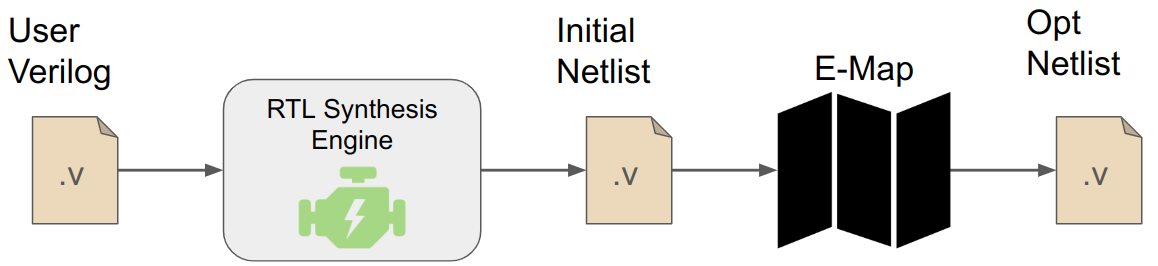
\includegraphics[width=0.47\textwidth]{img/flow.png}
    \caption{Tool flow to integrate E-Pack with existing RTL synthesis engines.}\label{fig:flow}
    \Description[]{}
\end{figure}

\subsection{Extraction}\label{sec:flow:extraction}
Regardless of whether equality saturation is achieved or not, the quality of
the output circuit still largely depends on the extraction technique used. In
short, \textit{extraction} is the process of selecting the ``best'' circuit
from the e-graph. Given that a saturated e-graph can contain hundreds of
thousands of e-nodes across tens of thousands of e-classes, a greedy extraction
algorithm is the most pragmatic. The greedy extractor iterates over the
e-classes, updating the cost of the cheapest e-node until the database of costs
no longer change. Whenever possible, our compiler uses the builtin
functionality of the egg e-graph Rust library~\cite{docsEgg}. However, e-graph
extraction itself is an ongoing research area~\cite{smoothe,
    sparsextract,esynth}, and future work would experiment with different
extraction algorithms. In any case, the cost of a LUT is always one plus the
sum of the costs of its children nodes. The subtle interactions between
extraction and the rewrite rule set are further explained in
Section~\todo{result sec}.

\subsection{Verilog Support}\label{sec:flow:verilog}
In order for our compiler to be compatible with as many existing design flows
as possible, some level of Verilog support is necessary. Our compiler supports
an ad-hoc subset of Verilog 2001~\cite{verilog}, as required to represent
structural netlists. This includes support for non-ANSI C style module
delcarations, wires, and module instantiations with named port connections.
With Verilog support, we are able to test \shortname{} with tool flows that use
Yosys~\cite{yosys} or Vivado~\cite{vivado}. On the backend, our compiler also
emits an updated Verilog netlist.

\subsection{Verification}\label{sec:flow:verification}
While verification is the not the primary focus of this work, some level of
validation is required to build trust in our synthesis results. In fact,
e-graphs were originally designed for automated theorem
proving~\cite{eggpaper}. Thus, constructing proofs that demonstrate equivalence
between the original and optimized netlist is a builtin feature of
\shortname{}. However, this technique is relatively slow, so we use two other
independent sources of verification. For combinational netlists, our middle end
can do exhaustive functional testing. Lastly, we use Yosys~\cite{yosys} for its
SAT-driven equivalence checking capabilities. All in all, the mixed usage of
these verification techniques build great confidence in the robustness of our
technology mapper built around e-graphs.
\section{Results}\label{sec:results}
For our experiments, we used a Red Hat 8 server running a Intel Xeon Gold 6242
CPU. Since \shortname{} is written in Rust, it mostly uses the built-in
functionality of the egg library. The egg e-graph runner was ran in a
time-limited configuration, meaning there was no limit in the size of the
e-graph or number of rewrite iterations. The specific time limit for e-graph
construction was 10 minutes. In most cases, the test circuit saturated the
e-graph before this time limit. \shortname{} was evaluated against circuits
from three benchmark suites: EPFL~\cite{epflbench}, ISCAS'85~\cite{iscasbench},
and LGSynth'91~\cite{lgsynthbench}. However, we also included an ALU and
pipelined multiplication module to test how our compiler behaves with
increasing levels of bit-parallelism and pipeline stages. Finally, we measure
how our mapping optimizations influence timing closure.

\subsection{Benchmarking}\label{sec:results:benchmark}
\begin{table}
    \centering
    \csvautobooktabular{data/results.csv}
    \caption{Results of 30 improved benchmarks from ISCAS'85, LGSynth'91, and EPFL}\label{tab:results}
\end{table}
Among the 96 benchmarks we tested, we found that \shortname{} was able to
reduce the LUT count 31\% of the time. On average, \shortname{} packed the
netlists to \metric{}. The results in Table~\ref{tab:results} list the LUT counts \todo{explain table}.

\subsection{Marginal Improvement}\label{sec:results:margin}
\todo{graph showing improvement with iter count}
\begin{figure}
    \centering
    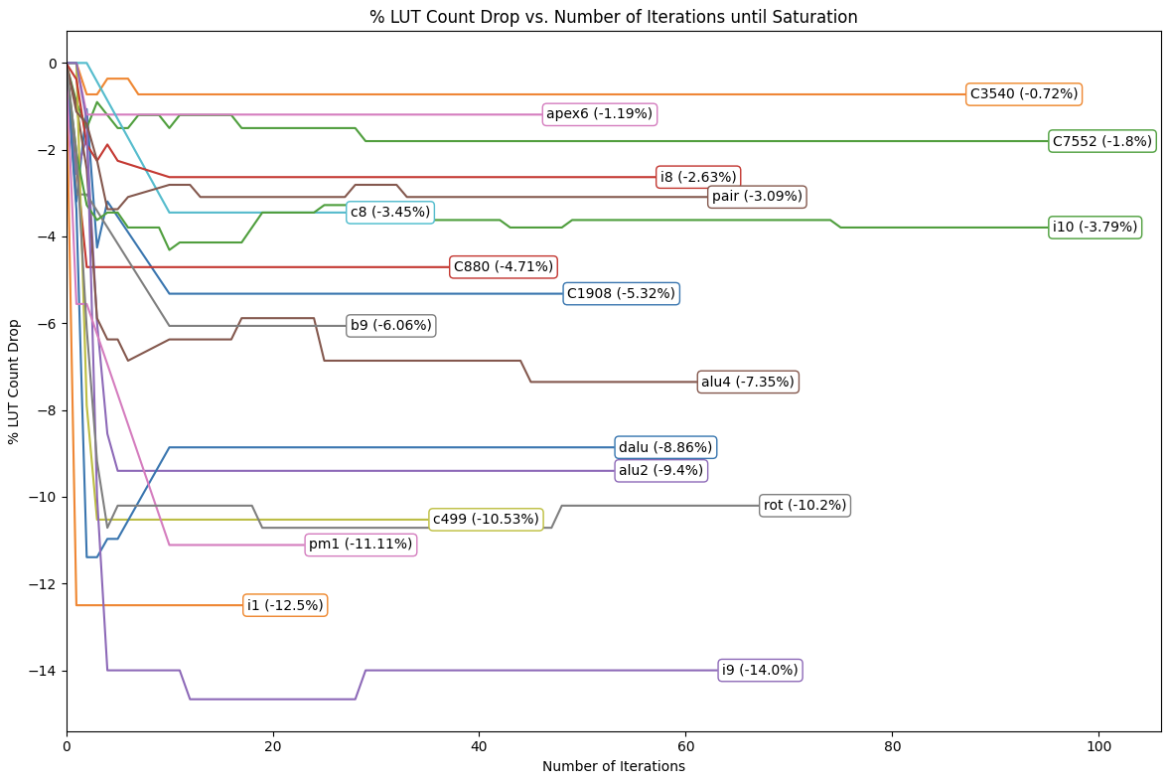
\includegraphics[width=0.47\textwidth]{img/improvement.png}
    \caption{Marginal improvement versus iteration count.}\label{fig:improvement}
    \Description[]{}
\end{figure}

\subsection{Pipelined Designs}\label{sec:results:retiming}
\todo{pipelined mult design}

\subsection{Bit-Parallel Designs}\label{sec:results:scalability}
\todo{increasing ALU bit parallelism}

\subsection{Runtime Complexity}\label{sec:results:complexity}
\todo{graph showing marginal runtime cost of each iteration}
\begin{figure}
    \centering
    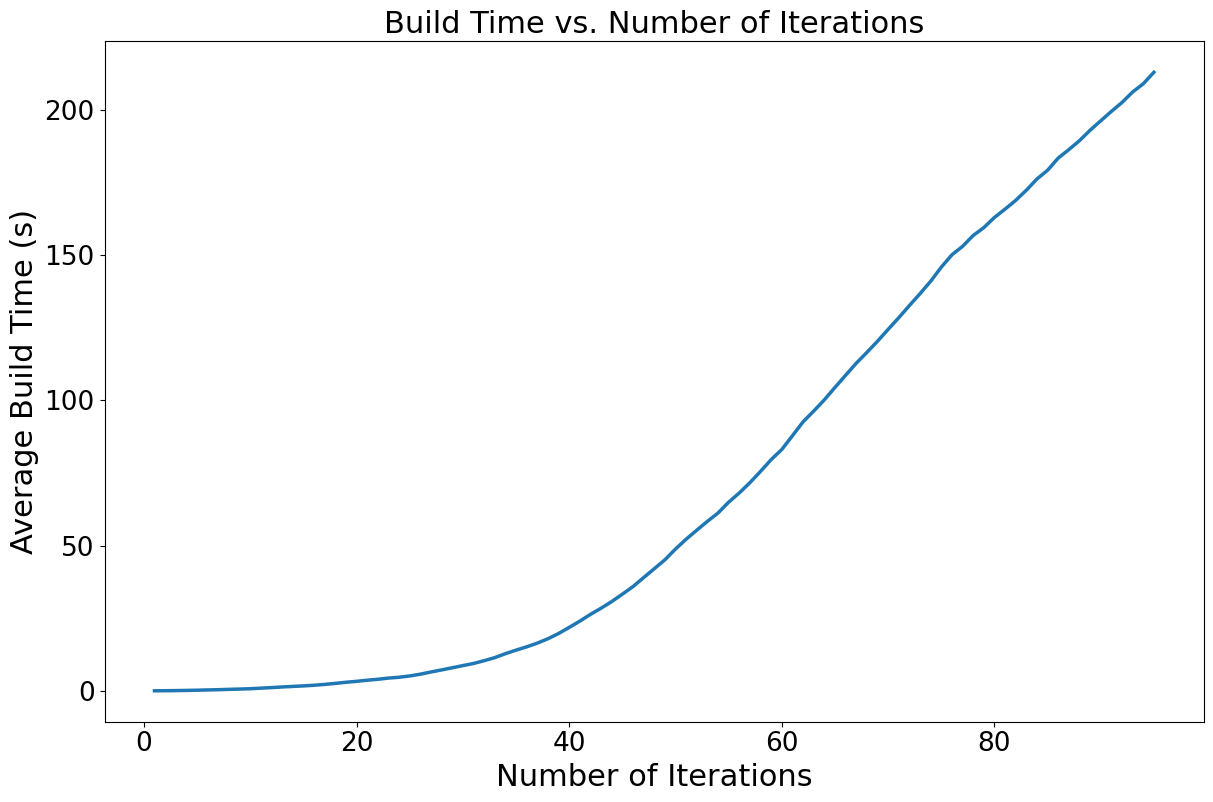
\includegraphics[width=0.47\textwidth]{img/runtime.png}
    \caption{Marginal increase in runtime versus iteration count.}\label{fig:runtime}
    \Description[]{}
\end{figure}

% Possible outline:
% 1. Related work
% 2. Egraph Construction
% 2.a. Simplifying degenerate LUTs
% 2.b. Functional composition
% 2.c. Functional decomposition
% 2.d. Symmetries of non-degenerate LUTs
% 2.e LUTs under restriction
% Experimental Setup
% results
% Future work

% use the ACM bibliography style
\bibliographystyle{ACM-Reference-Format}
\bibliography{references}

% \newpage
%%
%% If your work has an appendix, this is the place to put it.
% \appendix

\end{document}